
Nesse capítulo, será apresentado a construção do operador grosso Multiescala. A construção desse tipo de operador tem diversas aplicações para a solução dos sistemas lineares apresentados no capítulo \ref{ch:discretizacao}. Ele consiste basicamente em construir um operador grosso através do cálculo de funções de base em um grid gerado pelo acoplamento de elementos do grid fino. Pode ser utilizado como pré-condicionador \cite{casteletto}, como solver multinível semelhante aos solver multigrid ou ainda como aproximação para a solução original do problema. Os métodos multiescala tem sido aplicados com sucesso para problemas elípticos que é o caso do problema da elasticidade linear apresentado aqui. As vantagens do método apresentadas em \cite{thomashou} são que a funções de base multiescala tentam se adaptar as propriedades locais do operador de forma que o operador grosso as conserve, as funções de base podem ser construídas através da solução de problemas independentes e, portanto, em paralelo.

O primeiro passo para a construção do operador multiescala é gerar um novo grid com menos elementos que o grid original do problema (grid fino) que ainda representa o mesmo domínio $\Omega$. Esse grid novo será chamado de grid grosso e as variáveis relacionadas com ele serão assinadas com o sobre-escrito $H$. 
Assim grid grosso possui um conjunto $\tau_H$ de elementos onde cada elemento será uma aglomeração de elementos do grid fino. Por exemplo, a figura \ref{fig:gridgrosso} apresenta um grid grosso 3x3 construído a partir de um grid fino 7x7. É importante perceber que não existe a necessidade de aglomerar a mesma quantidade de elementos para se gerar o grid grosso já existem elementos formados por 9, 6 e 4 elementos do grid fino. Marcados de quadrados azuis estão mostrados os nós que pertencem ao grid grosso e grid fino.

\begin{figure}[!htbp]
\label{fig:gridgrosso}
\centering
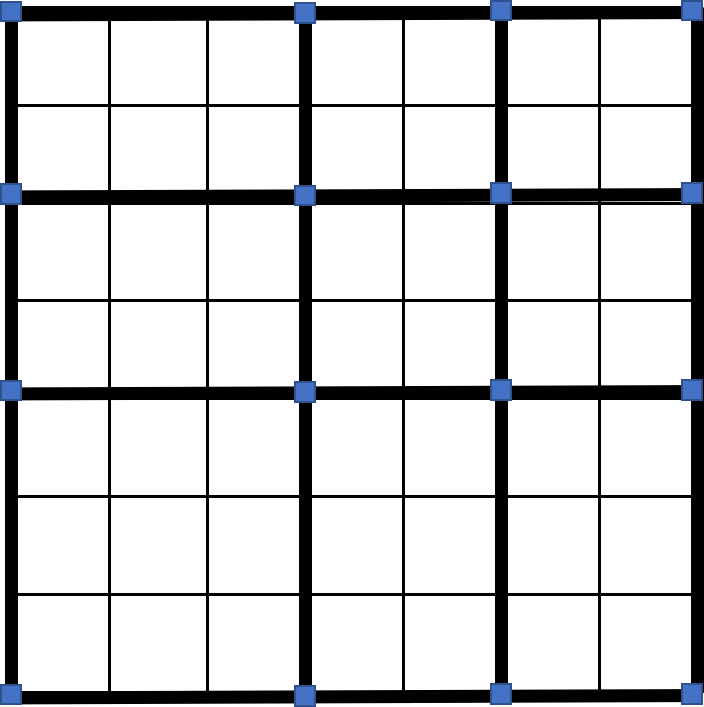
\includegraphics[width=6cm]{chap06/figs/grosso.png}
\caption{Exemplo de grid fino 7x7 e um grid grosso 3x3. O elemento inferior esquerdo é composto por 9 elementos do grid fino enquanto o elemento superior direito é composto com 4 elementos do grid fino.}
\end{figure}


No capítulo \ref{ch:discretizacao} foi apresentada a discretização através de elementos finitos para o problema de elasticidade linear através do método dos elementos finitos. A notação utilizada é baseada na utilizada em \cite{mbuck}. Assim, como naquele capítulo em que a função de desejada foi aproximada para um espaço $V^h$ formado por funções de base chapéu no domínio $\Omega$ do problema, a ideia agora é encontrar a solução do problema em um espaço grosso $V^{MS}$, tal que $V^{MS} \subset V^h$. 



Para definir melhor esse espaço $V^{MS}$ precisamos definir as suas funções de base geradoras. 


Novamente, para distinguir o nó pertencente ao grid grosso dos seus graus de liberdade o seguinte conjunto com graus de liberdade é criado.


\begin{equation}
    D^H = \{ p^{(m)} \in D^h : x^p \in \Sigma_H, m=1,2\}
\end{equation}


